%!TEX TS-program = ../make.zsh

\section{Experimental Background}
\label{sec:experimental_background}

\subsection{\icecube Detector}

The \icecube neutrino detector is built into a cubic-kilometer of the glacial ice at Earth's South Pole. 5160 photo detecting optical modules have been deployed between $1450\m$ and $2450\m$ below the surface. Construction has begun in 2005 with the deployment of the first optical modules. The detector is fully operational since 2010. \cite{instrumentation}

The optical modules are anchored on 86 vertical cables called \textit{strings}, which are positioned on a triangular grid with an overall hexagonal footprint. The strings are about $125\m$ apart. Each string holds 60 optical modules with a vertical spacing of $17\m$. \cite{instrumentation}

\begin{figure}[htbp]
  \smallerimage{icecube-schematics-instrumentation}
  \caption{Schematic overview of the \icecube detector. Image source: \cite{instrumentation}}
  \label{fig:aiThai0e}
\end{figure}

Additional to this \textit{in-ice array}, which is designed to measure neutrinos with energies from the TeV to the PeV scale, the \textit{DeepCore} sub array hold additional optical modules in order to lower the detection energy threshold in this region of the detector to detect neutrinos with energies from $10\GeV$ to $100\GeV$. \cite{instrumentation}


\subsection{Digital Optical Modules (DOMs)}
\label{sec:doms}

The basic detection unit in \icecube is the \textit{Digital Optical Module} (DOM). It consists of a glass sphere, a 10-inch photo multiplier tube (PMT), processing circuitry, and a flasher board with light-emitting diodes (LEDs) for calibration purposes (figure \ref{fig:aK4raigh}). \cite{instrumentation}

\begin{figure}[htbp]
  \subcaptionbox{The main components of the optical module are the photo multiplier tube (PMT), which detects impacting photons, the main electronics board that digitizes the signal and transmits the information to the surface, and the flasher board containing light-emitting diodes (LEDs) for calibration purposes. Image source: \cite{instrumentation}}{\halfimage{dom-components-instrumentation}}\hfill
  \subcaptionbox{The components of the module are contained within a glass sphere that can withstand high pressures. The space in between is filled with a gel to avoid optical effects at the medium boundaries. Image source: \cite{gallerynoharness}}{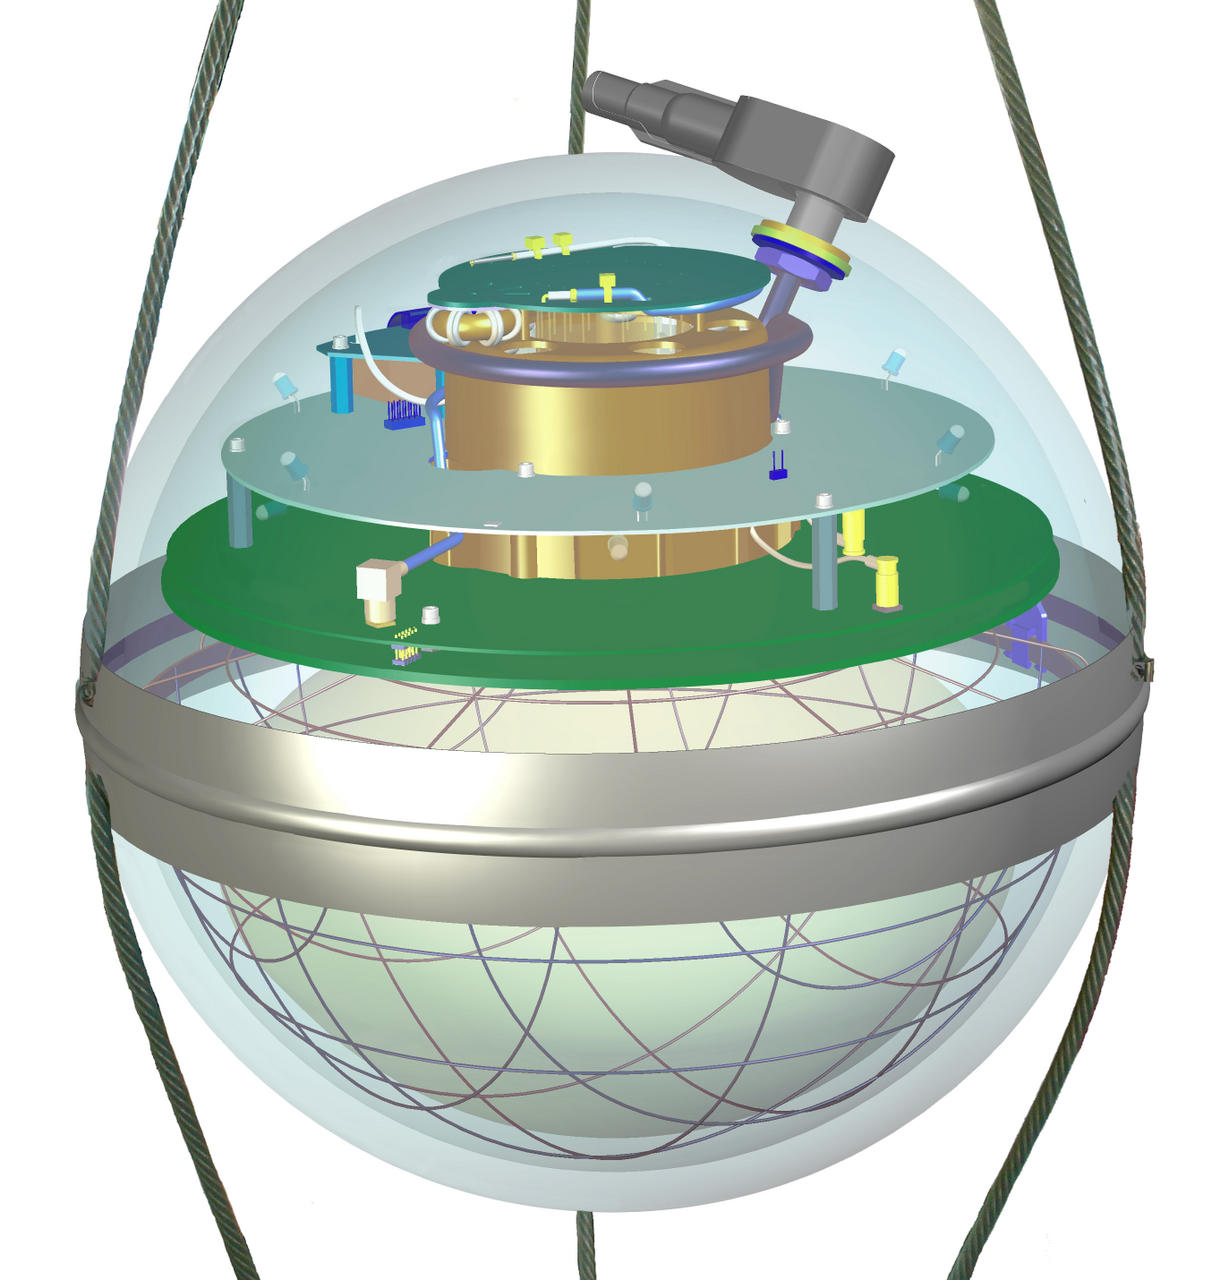
\includegraphics[width=0.35\textwidth]{img/DOMNoHarnessWhiteback_lg-gallery-2013}}
  \caption{Schematic display of a digital optical module (DOM), \icecube's basic detection unit. The module has an outer diameter of about $35\cm$. 5160 of these modules have been deployed in the glacial ice.}
  \label{fig:aK4raigh}
\end{figure}

% Other images:
% dom-8-top-hemisphere-and-penetrator-gallery-2011, source: Megan Madsen, 2011, https://gallery.icecube.wisc.edu/internal/v/GraphicRe/graphics/dom/8-top-hemisphere-and-penetrator.png.html
% dom-schematics-firstyearperformance, source: \cite{firstyearperformance}

The recorded signals from the PMT are digitized within the module before sending the signal to the surface in order to minimize the loss of information from degradation of analog signals sent over long distances. \cite{firstyearperformance}

The optical modules are optimized for detecting Cherenkov light emitted by particles with energies from $10\GeV$ to $10\PeV$ up to $500\m$ away from the optical module. \cite{instrumentation}


\subsection{Properties of South-Polar Ice}
\label{sec:ice}

The ice at the South Pole has exceptional optical properties, because air bubbles shrink and vanish under large pressure, forming a so-called \textit{clathrate hydrate}, where impurities are enclosed inside the ice crystal structure. \cite{rongenswedishcamera}

Using \icecube's LED flasher calibration system (section \ref{sec:doms}), the properties of \icecube's glacial ice have been measured: The average distance to absorption, $\lambda\abs$, the average distance between successive scatters $\lambda\sca$, and the angular distribution of the new direction after scattering. \cite{icepaper}

The ice has been divided into $z$-layers of an arbitrary thickness of $10\m$. The ice parameters have been fitted for each layer such that the properties are best interpreted as average of their true values over the thickness of the ice layers. \cite{icepaper}


\paragraph{Scattering}
The measured effective scattering lengths $\lambda\esca$ range from $5\m$ to $90\m$, corresponding to the geometric scattering length ranging from $0.3\m$ to $5.4\m$. The depth dependence of the scattering length is shown in figure \ref{fig:Ahxobai3} (a). \cite{icepaper}

\begin{figure}[htbp]
  \subcaptionbox{Depth dependence of the effective scattering length $\lambda\esca$. The effective scattering coefficient $b_\text{e}:=\sfrac{1}{\lambda\esca}$ is the inverse effective scattering length.}{\halfimage{icepaper-fig-16-esca}\vspace*{2mm}}\hfill
  \subcaptionbox{Depth dependence of the absorption length $\lambda\abs$. The absorption coefficient $a:= \sfrac{1}{\lambda\abs}$ is the inverse absorption length.}{\halfimage{icepaper-fig-16-abs}}
  \caption{Values of the absorption length $\lambda\abs$ and the effective scattering length $\lambda\esca$ for different depths, but for a fixed photon wave length of $400\nm$. Plot taken from \cite[figure 16]{icepaper}. A detailled data table is given in \cite[table C1]{icepaper}.}
  \label{fig:Ahxobai3}
\end{figure}

% - air bubble do not cause absorption, only scattering \cite{absorption1997}

The wave length dependence is given by equation \ref{eq:escawavelength} \cite[section 4]{icepaper}, where $b_\text{e} := \sfrac{1}{\lambda\esca}$ is the effective scattering coefficient, $\nu$ the photon wave length, and $\alpha$ a global fit parameter. $b_\text{e}(\nu = 400\nm)$ is given by figure \ref{fig:Ahxobai3} (a) and \cite[table C4]{icepaper}. The global parameter $\alpha$ has been fitted to $\alpha = 0.90 \pm 0.03$ \cite[section 5.1]{ackermann}.

\begin{equation}
  b_\text{e}(\nu) = b_\text{e}(\nu = 400\nm) \cdot \left(\frac{\nu}{400\nm}\right)^{-\alpha}
  \label{eq:escawavelength}
\end{equation}

The scattering prefers the forward direction, with a mean cosine of the scattering angle of $\meancostheta = 0.94$ \cite[paragraph 9]{ackermann} (or $\meancostheta = 0.90$ \cite{icepaper}).


\paragraph{Absorption}
The absorption lengths in the South-Polar ice vary between $10\m$ in dusty regions and $280\m$ in very clear ice layers. Their depth dependence is given in figure \ref{fig:Ahxobai3} (b). The absorption length, which is governed by the dust concentration, is especially low in the so-called ``dust peak'' at a depth of about $2000\m$. \cite{ackermann, ppcpaper, icepaper}

The dependence of the absorption coefficient $a := \sfrac{1}{\lambda\abs}$ on the photon wave length $\nu$, the temperature difference $\delta\tau$ is given by equation \ref{eq:abswavelength} \cite{icepaper}.

\begin{equation}
  a(\nu) = a_\text{dust}(\nu) + A\,\e^{-\sfrac{B}{\nu}}\, (1 + 0.01 \cdot \delta\tau)
  \label{eq:abswavelength}
\end{equation}
\begin{equation}
  a_\text{dust}(\nu) = a_\text{dust}(\nu = 400\nm) \left(\frac{\nu}{400\nm}\right)^{-\kappa}
\end{equation}

The global parameters have been fitted to $A = (6954 \pm 973)\m^{-1}$, $B = (6618 \pm 71)\nm$, and $\kappa = 1.08 \pm 0.01$ \cite[section 5.2]{ackermann}.\footnote{The quantity $A$ in \cite{icepaper} corresponds to the quantity $A_\text{IR}$ in \cite{ackermann}. $B$ in \cite{icepaper} corresponds to $\lambda_0$ in \cite{ackermann}.}
The temperature difference $\delta\tau(d) = T(d) - T(1730\m)$ for depths $d$ is given by equation \ref{eq:temperature} \cite{icepaper}.

\begin{equation}
  T(d) = 221.5\unit{K} - 0.00045319\,\frac{\text{K}}{\text{m}}\cdot d + 5.822 \cdot 10^{-6}\,\frac{\text{K}}{\text{m}^2} \cdot d^2
  \label{eq:temperature}
\end{equation}


\paragraph{Ice-Layer Tilt and Ice Anisotropy}
The absorption properties of the ice layers follow the dust concentration, which does not strictly follow the arbitrary $z$-layers, but is tilted. To model this feature, the ice layers can also be tilted by using an effective-$z$ coordinate, $z_\text{e}(x,y,z) = z + \text{relief}(x,y,z)$, which is shown in figure \ref{fig:wohr8uaY}. \cite{icepaper}

\begin{figure}[htbp]
  \centering
  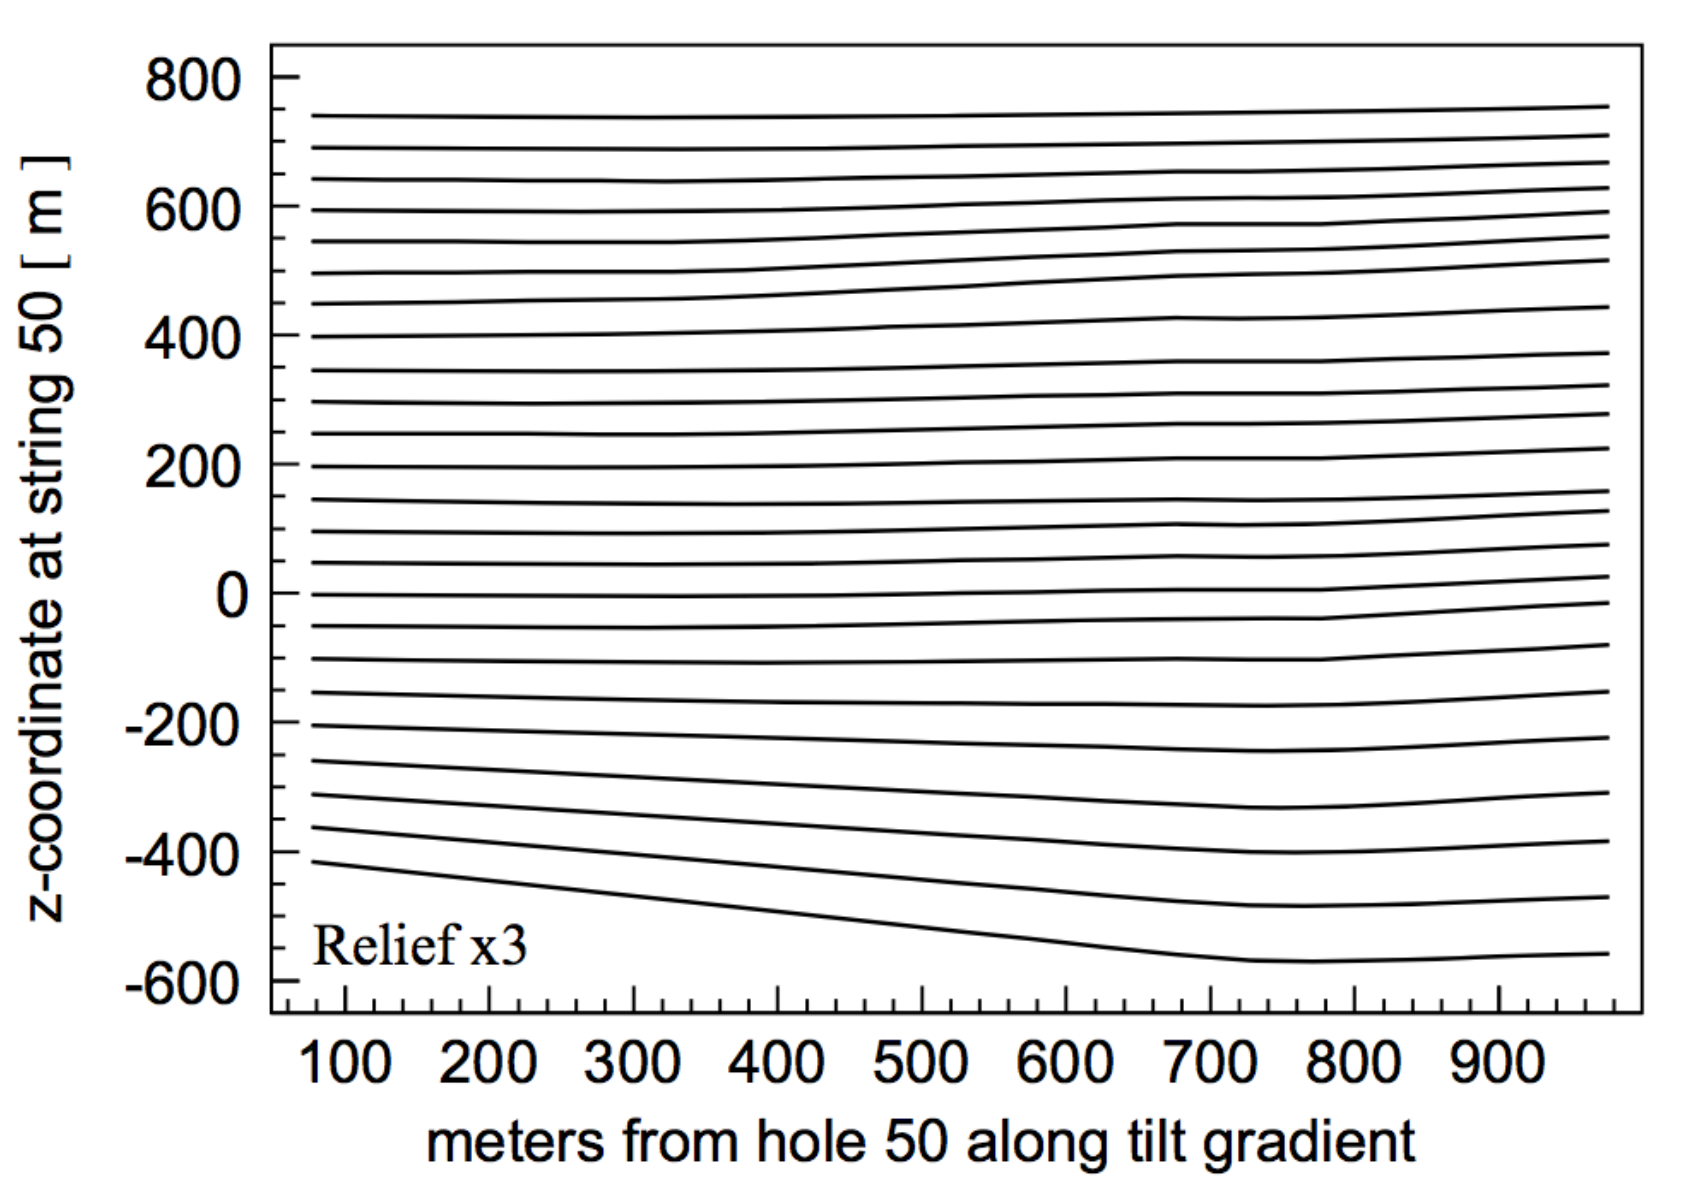
\includegraphics[width=0.5\textwidth]{img/icepaper-fig-14-layers}
  \caption{Ice layers along the average gradient direction within the ice. The relief is amplified by a factor of 3 to enhance the clarity of the layer structure. The lowest layer shown exhibits a shift of $56\m$ betweeen its shallowest and deepest points, which is the largest shift of all layers shown in the figure. Plot and caption taken from \cite[figure 14]{icepaper}.}
  \label{fig:wohr8uaY}
\end{figure}

Furthermore, scattering and absorption show also a slight dependency on the propagation direction of the photons, aligned with the ice flow direction of the glacier. \cite{icrc17pocam}

This study considers the dependencies of scattering and absorption length on depth, temperature and wavelength, but does not consider the ice-layer tilt and the ice anisotropy.

An overview of the different ice models used in \icecube is given in \cite{flasherdataderivedicemodels}.


\subsection{Hole Ice Around the Detector Strings}
\label{sec:hole_ice}

The so-called \textit{hole ice} is the refrozen water within the drill holes that were necessary to deploy the detector strings with the optical modules.

For the \icecube detector, 68 boreholes with an approximate diameter of $60\cm$ to a depth of about $2500\m$ were created using a \textit{hot-water drilling} technique. Drilling one hole required about 48 hours time. \cite{instrumentation}

When the glacial ice in the drill holes became water, the structures that were responsible for the specific properties of the bulk-ice layers were destroyed. Thus, the properties of the hole ice are considered largely independent of those of the surrounding bulk ice. The deployed instrumentation become frozen in place and optically coupled to the surrounding ice sheet when the water in the boreholes became ice again. \cite{instrumentation}

In order to monitor the freeze-in process, a camera system consisting of two video cameras in separate spheres, each also equipped with four LEDs and three lasers, has been deployed along one of the detector strings. The cameras observed that the drill hole became completely refrozen within 15 days. \cite{instrumentation}

The camera observations suggest two hole-ice components, a clear outer region, and an inner column of a smaller scattering length and a diameter of about $16\cm$ (figure \ref{fig:daeM6yot}). \cite{rongenswedishcamera,instrumentation}

\begin{figure}[htbp]
  \centering
  \subcaptionbox{}{\thirdimage{camera2010-01}}\hfill
  \subcaptionbox{}{\thirdimage{camera2010-02}}\hfill
  \subcaptionbox{}{\thirdimage{camera2010-03}}\hfill
  \subcaptionbox{}{\thirdimage{camera2010-04}}\hfill
  \subcaptionbox{}{\thirdimage{camera2010-05}}\hfill
  \subcaptionbox{}{\thirdimage{camera2010-06}}\hfill
  \subcaptionbox{}{\halfimage{swedish-camera-downwards}}\hfill
  \subcaptionbox{}{\halfimage{camera2018-01}}\hfill
  \caption{Monitoring the freeze-in process using a camera system deployed within string number 80. The drill hole freezes from outside in as seen in (a) to (f). The final configuration that can still be observed in 2018 as seen in (h) still shows a diffuse column, called \enquote{bubble column}, on the right-hand side of images (g) and (h). Image sources: \cite{icrc17pocam, camera2010, camera2018}}
  \label{fig:daeM6yot}
\end{figure}

The observed freeze-in process from the outside in is consistent with the theory of \textit{cylindrical freezing}, where impurities or air bubbles are pushed inwards along the freezing boundaries until they merge in the center. \cite{rongenswedishcamera} After completing the freeze-in process, no long-term changes have been observed from 2010 to 2018. \cite{instrumentation, camera2010, camera2018}

In this study, when needing to differenciate between the different components of the hole ice, the outer clear component will be called \textit{drill-hole ice}, or \textit{drill-hole column}. The inner component with a shorter scattering length will be called \textit{bubble column}. Note, however, that there is no established nomenclature in the context of \icecube publications, yet.

In this study, the hole-ice columns will be modeled as cylinders. More complicated geometries such as accounting for the inevitable swinging of the drilling head, or pressure effects that could lead to a vertial gradient in the properties of the hole ice, are not subject of this study.\followup

